\section{Work}\label{sec:work}

\textit{Work} is the scientific term used to describe the action of a force which moves an object. When a constant force $F$ is applied to move an object a distance $d$, the amount of work performed is $W=F\cdot d$. 

The SI unit of force is the Newton, (kg$\cdot$m/s$^2$), and the SI unit of distance is a meter (m). The fundamental unit of work is one Newton-meter, or a Joule (J). That is, applying a force of one Newton for one meter performs one Joule of work. In Imperial units (as used in the United States), force is measured in pounds (lb) and distance is measured in feet (ft), hence work is measured in ft-lb. 

\mnote{\textbf{Note:} \textit{Mass} and \textit{weight} are closely related, yet different, concepts. The mass $m$ of an object is a quantitative measure of that object's resistance to acceleration. The weight $w$  of an object is a measurement of the force applied to the object by the acceleration of gravity $g$.\\

Since the two measurements are proportional, $w=m\cdot g$, they are often used interchangeably in everyday conversation. When computing work, one must be careful to note which is being referred to. When mass is given, it must be multiplied by the acceleration of gravity to reference the related force.}

When force is constant, the measurement of work is straightforward. For instance, lifting a 200 lb object 5 ft performs $200\cdot 5 = 1000$ ft-lb of work. 

What if the force applied is variable? For instance, imagine a climber pulling a 200 ft rope up a vertical face. The rope becomes lighter as more is pulled in, requiring less force and hence the climber performs less work.

In general, let $F(x)$ be a force function on an interval $[a,b]$. We want to measure the amount of work done applying the force $F$ from $x=a$ to $x=b$. We can approximate the amount of work being done by partitioning $[a,b]$ into subintervals $a=x_0<x_1 <\dots <x_n=b$ and assuming that $F$ is constant on each subinterval. Let $c_i$ be a value in the $i\,^{\text{th}}$ subinterval $[x_i,x_{i+1}]$. Then the work done on this interval is approximately $W_i\approx F(c_i)\cdot(x_{i+1}-x_i) = F(c_i)\Delta x_i$, a constant force $\times$ the distance over which it is applied. The total work is 
\[ W = \sum_{i=1}^n W_i \approx \sum_{i=1}^n F(c_i)\Delta x_i.\]
This, of course, is a Riemann sum. Taking a limit as the subinterval lengths go to zero give an exact value of work which can be evaluated through a definite integral.

\keyidea{idea:work}{Work}
{Let $F(x)$ be a continuous function on $[a,b]$ describing the amount of force being applied to an object in the direction of travel from distance $x=a$ to distance $x=b$. The total work $W$ done on $[a,b]$ is
\index{integration!work}\index{work}
\[W = \int_a^b F(x)\ dx.\]}

\youtubeVideo{2pbInn9PkHQ}{Finding Work using Calculus --- The Cable/Rope Problem}

\example{ex_work1}{Computing work performed: applying variable force}{%
A 60 m climbing rope is hanging over the side of a tall cliff. How much work is performed in pulling the rope up to the top, where the rope has a mass of 66 g/m? 
%How much work is performed pulling a 60 m climbing rope up a cliff face, where the rope has a mass of 66 g/m?
}
{We need to create a force function $F(x)$ on the interval $[0,60]$. To do so, we must first decide what $x$ is measuring: is it the length of the rope still hanging or is it the amount of rope pulled in? As long as we are consistent, either approach is fine. We adopt for this example the convention that $x$ is the amount of rope pulled in. This seems to match intuition better; pulling up the first 10 meters of rope involves $x=0$ to $x=10$ instead of $x=60$ to $x=50$. 

As $x$ is the amount of rope pulled in, the amount of rope still hanging is $60-x$. This length of rope has a mass of 66 g/m, or $0.066$ kg/m. The the mass of the rope still hanging is $0.066(60-x)$ kg; multiplying this mass by the acceleration of gravity, 9.8 m/s$^2$, gives our variable force function
\[F(x) = (9.8)(0.066)(60-x) = 0.6468(60-x).\]

Thus the total work performed in pulling up the rope is 
\[W = \int_0^{60} 0.6468(60-x)\ dx = 1,164.24\ \text{J}.\]

By comparison, consider the work done in lifting the entire rope 60 meters. The rope weights $60\times 0.066 \times 9.8 = 38.808$ N, so the work applying this force for 60 meters is $60\times 38.808 = 2,328.48$ J. This is exactly twice the work calculated before (and we leave it to the reader to understand why.)}

\example{ex_work1_5}{Computing work performed: applying variable force}{Consider again pulling a 60 m rope up a cliff face, where the rope has a mass of 66 g/m. At what point is exactly half the work performed?}
{From \autoref{ex_work1} we know the total work performed is $1,164.24$ J. We want to find a height $h$ such that the work in pulling the rope from a height of $x=0$ to a height of $x=h$ is 582.12, half the total work. Thus we want to solve for $h$ in the equation
\[\int_0^h 0.6468(60-x)\ dx = 582.12.\]

We see that
\begin{align*}
	\int_0^h 0.6468(60-x)\ dx &= 582.12 \\
	\left(38.808x-0.3234x^2\right)\Big|_0^h &=582.12 \\
	38.808h-0.3234h^2 &=582.12 \\
	-0.3234h^2+38.808h-582.12 &=0 \qquad\qquad\text{\small(Apply the Quadratic Formula)} \\
%\intertext{Apply the Quadratic Formula.}
	h&\approx17.57 \ \text{and}\ 102.43
\end{align*}
\mnote{\textbf{Note:} In \autoref{ex_work1_5}, we find that half of the work performed in pulling up a 60 m rope is done in the last 42.43 m. Why is it not coincidental that $60/\sqrt{2}=42.43$?}
As the rope is only 60m long, the only sensible answer is $h=17.57$. Thus about half the work is done pulling up the first 17.57m the other half of the work is done pulling up the remaining 42.43m.}

\example{ex_work2}{Computing work performed: applying variable force}{A box of 100 lb of sand is being pulled up at a uniform rate a distance of 50 ft over 1 minute. The sand is leaking from the box at a rate of 1 lb/s. The box itself weighs 5 lb and is pulled by a rope weighing .2 lb/ft. 
\begin{enumerate}
	\item	How much work is done lifting just the rope?
	\item	How much work is done lifting just the box and sand?
	\item	What is the total amount of work performed?
\end{enumerate}}
{\begin{enumerate}
	\item	We start by forming the force function $F_r(x)$ for the rope (where the subscript denotes we are considering the rope). As in the previous example, let $x$ denote the amount of rope, in feet, pulled in. (This is the same as saying $x$ denotes the height of the box.) The weight of the rope with $x$ feet pulled in is $F_r(x) = 0.2(50-x) = 10-0.2x$. (Note that we do not have to include the acceleration of gravity here, for the \textit{weight} of the rope per foot is given, not its \textit{mass} per meter as before.) The work performed lifting the rope is 
	\[W_r = \int_0^{50} (10-0.2x)\ dx = 250\ \text{ft-lb}.\]
	
	\item	The sand is leaving the box at a rate of 1 lb/s. As the vertical trip is to take one minute, we know that 60 lb will have left when the box reaches its final height of 50 ft. Again letting $x$ represent the height of the box, we have two points on the line that describes the weight of the sand: when $x=0$, the sand weight is 100 lb, producing the point $(0,100)$; when $x=50$, the sand in the box weighs 40 lb, producing the point $(50,40)$. The slope of this line is $\frac{100-40}{0-50} = -1.2$, giving the equation of the weight of the sand at height $x$ as $w(x) = -1.2x+100$. The box itself weighs a constant 5 lb, so the total force function is $F_b(x) = -1.2x+105$. Integrating from $x=0$ to $x=50$ gives the work performed in lifting box and sand:
	\[W_b = \int_0^{50} (-1.2x+105)\ dx = 3750\ \text{ft-lb.}\]
	
	\item	The total work is the sum of $W_r$ and $W_b$: $250+3750=4000$ ft-lb. We can also arrive at this via integration:
	\begin{align*}
	W
	&= \int_0^{50} (F_r(x)+F_b(x))\ dx \\
	&= \int_0^{50} (10-0.2x-1.2x+105)\ dx \\
	&= \int_0^{50} (-1.4x+115) \ dx \\
	&= 4000 \ \text{ft-lb.}\eoehere
	\end{align*}	
\end{enumerate}}

\subsection{Hooke's Law and Springs}

Hooke's Law states that the force required to compress or stretch a spring $x$ units from its natural length is proportional to $x$; that is, this force is $F(x) = kx$ for some constant $k$. For example, if a force of 1 N stretches a given spring 2 cm, then a force of 5 N will stretch the spring 10 cm. Converting the distances to meters, we have that stretching this spring 0.02 m requires a force of $F(0.02) = k(0.02) = 1$ N, hence $k = 1/0.02 = 50$ N/m. 
\index{Hooke's Law}

\example{ex_spring1}{Computing work performed: stretching a spring}{A force of 20 lb stretches a spring from a natural length of 7 inches to a length of 12 inches. How much work was performed in stretching the spring to this length?}
{In many ways, we are not at all concerned with the actual length of the spring, only with the amount of its change. Hence, we do not care that 20 lb of force stretches the spring to a length of 12 inches, but rather that a force of 20 lb stretches the spring by 5 in. This is illustrated in \autoref{fig:spring1}; we only measure the change in the spring's length, not the overall length of the spring.

\begin{figure}[!hb]
\centering
\begin{tikzpicture}
 \begin{scope}[xscale=.2,yscale=.5,shift={(.5,0)}]
  \draw [thick,draw={\colorone}] (-1,.5)--(-.5,.5)--(0,0);
  \foreach \x in {0,1,...,5} {
   \begin{scope}[shift={(\x*2,0)}]
    \draw [thick,draw={\colorone}] (0,0)--(1,1)--(2,0);
   \end{scope}
  }
  \begin{scope}[shift={(12,0)}]
   \draw [thick,draw={\colorone}] (0,0) --(1,1) --(1.5,.5)--(2,.5);
  \end{scope}
 \end{scope}
 \draw [shift={(.9,0)},thick,left color={\colorone!70},right color={\coloronefill},{\colorone}] (2,0) rectangle (2.5,.5);
 \draw [shift={(.9,0)},->,>=stealth]
  (2.75,.15)-= node [pos=.5,above] {$F$} (3.25,.15);
 \begin{scope}[shift={(0,-.25)}]
  \draw [thick] (-.5,0)--(5.5,0);
  \foreach \x in {0,...,6} {
   \draw (\x*.4+2.8,.1)--(\x*.4+2.8,-.1) node [below] {\scriptsize $\x$};
  }
 \end{scope}
 \begin{scope}[shift={(0,-1.75)}]
  \begin{scope}[xscale=.343,yscale=.5,shift={(.5,0)}]
   \draw [thick,draw={\colorone}] (-1,.5)--(-.5,.5)--(0,0);
   \foreach \x in {0,1,...,5} {
    \begin{scope}[shift={(\x*2,0)}]
     \draw [thick,draw={\colorone}] (0,0)--(1,1)--(2,0);
    \end{scope}
   }
   \begin{scope}[shift={(12,0)}]
    \draw [thick,draw={\colorone}] (0,0) --(1,1) --(1.5,.5)--(2,.5);
   \end{scope}
  \end{scope}
  \begin{scope}[shift={(0,-.25)}]
   \draw [thick] (-.5,0)--(5.5,0);
   \foreach \x in {0,...,6} {
    \draw (\x*.4+2.8,.1)--(\x*.4+2.8,-.1) node [below] {\scriptsize $\x$};
   }
  \end{scope}
  \draw [shift={(2.9,0)},thick,left color={\colorone!70},right color={\coloronefill},{\colorone}] (2,0) rectangle (2.5,.5);
 \end{scope}             
\end{tikzpicture}
\caption{Illustrating the important aspects of stretching a spring in computing work in \autoref{ex_spring1}.}
\label{fig:spring1}
\end{figure}

Converting the units of length to feet, we have
\[F(5/12) = (5/12)k = 20\ \text{lb}.\]
Thus $k = 48$ lb/ft and $F(x) = 48x$. 

We compute the total work performed by integrating $F(x)$ from $x=0$ to $x=5/12$:
\begin{align*}
	W
	&= 	\int_0^{5/12} 48x \ dx \\
	&=	24x^2\Big|_0^{5/12} \\
	&=  25/6 %\approx 4.1667
	\ \text{ft-lb.}\eoehere
\end{align*}}

\subsection{Pumping Fluids}

\mtable[-.5in]{Weight and Mass densities}{fig:weight_density}{%
\begin{tabular}{lll}
Fluid & lb/ft$^3$ & kg/m$^3$ \\ \midrule
Gasoline & \phantom{0}45.93 & \phantom{00}737.22\\
Methanol & \phantom{0}49.3 & \phantom{00}791.3\\
Fuel Oil & \phantom{0}55.46 & \phantom{00}890.13 \\
Water & \phantom{0}62.4 & \phantom{0}1000 \\
Milk, whole & \phantom{0}63.6 & \phantom{0}1020 \\
Milk, nonfat & \phantom{0}65.4 & \phantom{0}1050 \\
Concrete & 150 & \phantom{0}2400 \\
Iodine & 307 & \phantom{0}4927 \\
Mercury & 844 & 13546
\end{tabular}}

Another useful example of the application of integration to compute work comes in the pumping of fluids, often illustrated in the context of emptying a storage tank by pumping the fluid out the top. This situation is different than our previous examples for the forces involved are constant. After all, the force required to move one cubic foot of water (about 62.4 lb) is the same regardless of its location in the tank. What is variable is the distance that cubic foot of water has to travel; water closer to the top travels less distance than water at the bottom, producing less work.

We demonstrate how to compute the total work done in pumping a fluid out of the top of a tank in the next two examples.

\example{ex_pump1}{Computing work performed: pumping fluids}{A cylindrical storage tank with a radius of 10 ft and a height of 30 ft is filled with water, which weighs approximately 62.4 lb/ft$^3$. Compute the amount of work performed by pumping the water up to a point 5 feet above the top of the tank.}
{We will refer often to \autoref{fig:pump1a} which illustrates the salient aspects of this problem.

\mtable{Illustrating a water tank in order to compute the work required to empty it in \autoref{ex_pump1}.}{fig:pump1a}{\begin{tikzpicture}[x=.1cm,y=.125cm,>=stealth]
\draw [->] (0,-2) -- (0,37) node [above] {\scriptsize $y$};
\draw (-1,0) node [left] {\scriptsize 0} -- (1,0)
      (-1,30) node [left] {\scriptsize 30} -- (1,30)
      (-1,35) node [left] {\scriptsize 35} -- (1,35);
\draw (2,12)--(4,12)  (2,35)--(4,35)
      (3,12) -- node [pos=.5,fill=white,rotate=90] {\scriptsize $35-y_i$} (3,35);
\begin{scope}[xscale=4,shift={(4.5,0)}]         
\draw (0,30) -- node [pos=.5,above] {\scriptsize $10$} (2.9,29.22);             
\draw [thick] (3,30) --(3,0) arc (0:-180:3) -- (-3,30);
\draw [thick](0,30) circle (3);
\draw [thick,dashed] (3,0) arc (0:180:3);
\foreach \y/\x in {12/{$y_i$},16/{$y_{i+1}$}} {
	\draw (3,\y) node [right] {\scriptsize\x} arc (0:-180:3);
    \draw [dashed] (3,\y) arc (0:180:3);
}
\draw (5.1,14) node {\scriptsize $\left.\rule{0pt}{.3cm}\right\}\Delta y_i$};
\draw [left color={\colorone},right color={\coloronefill},thick] (0,16) circle (3);
\draw [left color={\colorone},right color={\coloronefill},thick]
 (-3,16) -- (-3,12)  arc (180:360:3) -- (3,16) arc (360:180:3);
\end{scope}
\end{tikzpicture}}
% todo Tim make the water tank figure into 3d?

We start as we often do: we partition an interval into subintervals. We orient our tank vertically since this makes intuitive sense with the base of the tank at $y=0$. Hence the top of the water is at $y=30$, meaning we are interested in subdividing the $y$-interval $[0,30]$ into $n$ subintervals as 
\[0 = y_0 < y_1 < \dots < y_n = 30.\]
Consider the work $W_i$ of pumping only the water residing in the $i\,^\text{th}$ subinterval, illustrated in \autoref{fig:pump1a}. The force required to move this water is equal to its weight which we calculate as volume $\times $ density. The volume of water in this subinterval is 
$V_i = 10^2\pi \Delta y_i$; its density is $62.4$ lb/ft$^3$. Thus the required force is $6240\pi\Delta y_i$ lb.

We approximate the distance the force is applied by using any $y$-value contained in the $i\,^\text{th}$ subinterval; for simplicity, we arbitrarily use $y_i$ for now (it will not matter later on). The water will be pumped to a point 5 feet above the top of the tank, that is, to the height of $y=35$ ft. Thus the distance the water at height $y_i$ travels is $35-y_i$ ft. 

In all, the approximate work $W_i$ peformed in moving the water in the $i\,^\text{th}$ subinterval to a point 5 feet above the tank is 
\[W_i \approx 6240\pi\Delta y_i(35-y_i).\]
To approximate the total work performed in pumping out all the water from the tank, we sum all the work $W_i$ performed in pumping the water from each of the $n$ subintervals of $[0,30]$:
\[W \approx \sum_{i=1}^n W_i = \sum_{i=1}^n 6240\pi\Delta y_i(35-y_i).\]
This is a Riemann sum. Taking the limit as the subinterval length goes to 0 gives 
\begin{align*}
W 	&=	\int_0^{30} 6240\pi(35-y)\ dy \\
		&=  6240\pi\left(35y-\frac{y^2}2\right)\Big|_0^{30} \\
		&= 	11,762,123 \ \text{ft-lb}\\
		&\approx  1.176 \times 10^7 \ \text{ft-lb}.\eoehere
\end{align*}}

\mtable{A simplified illustration for computing work.}{fig:pump1b}{\begin{tikzpicture}[x=.1cm,y=.125cm,>=stealth]
\draw [->] (0,-2) -- (0,37) node [above] {\scriptsize $y$};
\draw (-1,0) node [left] {\scriptsize 0} -- (1,0)
      (-1,30) node [left] {\scriptsize 30} -- (1,30)
      (-1,35) node [left] {\scriptsize 35} -- (1,35)
      (-1,14) node [left] {\scriptsize $y$} -- (1,14);
\draw (2,14)--(4,14)  (2,35)--(4,35)
      (3,14) -- node [pos=.5,fill=white,rotate=90] {\scriptsize $35-y$} (3,35);
\begin{scope}[xscale=4,shift={(4.5,0)}]         
\draw (0,30) -- node [pos=.5,above] {\scriptsize $10$} (2.9,29.22);                             
\draw [thick](3,30) --(3,0) arc (0:-180:3) -- (-3,30);
\draw [thick] (0,30) circle (3);
\draw [thick,dashed] (3,0) arc (0:180:3);
\draw [left color={\colorone},right color={\coloronefill},thick,draw={\colorone}] (0,14) circle (3);
\draw [->] (5.25,16) node [above] {\scriptsize $V(y)=100\pi dy$} -- (2,14);
\end{scope}
\end{tikzpicture}}
% todo Tim make the simplified water tank into 3d?

We can ``streamline'' the above process a bit as we may now recognize what the important features of the problem are. \autoref{fig:pump1b} shows the tank from \autoref{ex_pump1} without the $i\,^\text{th}$ subinterval identified. Instead, we just draw a sample slice. This helps establish the height a small amount of water must travel along with the force required to move it (where the force is volume $\times$ density).

We demonstrate the concepts again in the next examples.

\example{ex_pump2}{Computing work performed: pumping fluids}{A conical water tank has its top at ground level and its base 10 feet below ground. The radius of the cone at ground level is 2 ft. It is filled with water weighing 62.4 lb/ft$^3$ and is to be emptied by pumping the water to a spigot 3 feet above ground level. Find the total amount of work performed in emptying the tank.}
{The conical tank is sketched in \autoref{fig:pump2}. We can orient the tank in a variety of ways; we could let $y=0$ represent the base of the tank and $y=10$ represent the top of the tank, but we choose to keep the convention of the wording given in the problem and let $y=0$ represent ground level and hence $y=-10$ represents the bottom of the tank. The actual ``height'' of the water does not matter; rather, we are concerned with the distance the water travels. 

\mtable[-.5in]{A graph of the conical water tank in \autoref{ex_pump2}.}{fig:pump2}{\begin{tikzpicture}[x=.1cm,y=.125cm,>=stealth]
\draw [->] (0,-2) -- (0,37) node [above] {\scriptsize $y$};
\draw (-1,0) node [left] {\scriptsize $-10$} -- (1,0)
      (-1,30) node [left] {\scriptsize 0} -- (1,30)
      (-1,35) node [left] {\scriptsize 3} -- (1,35)
      (-1,14) node [left] {\scriptsize $y$} -- (1,14);
\draw (2,14)--(4,14)  (2,35)--(4,35)
      (3,14) -- node [pos=.5,fill=white,rotate=90] {\scriptsize $3-y$} (3,35);
\begin{scope}[xscale=4,shift={(4.5,0)}]         
\draw (0,30) -- node [pos=.5,above] {\scriptsize $2$} (2.9,29.22);                              
\draw [thick](3,30) --(0,0) -- (-3,30);
\draw [thick] (0,30) circle (3);
\draw [left color={\colorone},right color={\coloronefill},thick,draw={\colorone}] (0,14) circle (1.4);
\draw [->] (3.4,6) node [below] {\scriptsize $V(y)=\pi(\frac y5+2)^2 dy$} -- (0,14);
\end{scope}
\end{tikzpicture}}
% todo Tim make the water cone into 3d?

The figure also sketches %a differential element,
a cross-sectional circle. The radius of this circle is variable, depending on $y$. When $y=-10$, the circle has radius 0; when $y=0$, the circle has radius 2. These two points, $(-10,0)$ and $(0,2)$, allow us to find the equation of the line that gives the radius of the cross-sectional circle, which is $r(y) = y/5+2$. Hence the volume of water at this height is $V(y)=\pi(y/5+2)^2dy$, where $dy$ represents a very small height of the slice. The force required to move the water at height $y$ is $F(y) = 62.4\times V(y)$.

The distance the water at height $y$ travels is given by $h(y)=3-y$. Thus the total work done in pumping the water from the tank is 
\begin{align*}
	W
	&= \int_{-10}^0 62.4\pi(y/5+2)^2(3-y)\ dy\\
	&= 62.4\pi\int_{-10}^0\left(-\frac1{25}y^3-\frac{17}{25}y^2-\frac85y+12\right)\ dy\\
	&= 62.2\pi\cdot\frac{220}{3} %\approx 14,376
	\text{ ft-lb.}	\eoehere
\end{align*}}

\example{ex_pump3}{Computing work performed: pumping fluids}{A rectangular swimming pool is 20 ft wide and has a 3 ft ``shallow end'' and a 6 ft ``deep end.'' It is to have its water pumped out to a point 2 ft above the current top of the water. 
The cross-sectional dimensions of the water in the pool are given in \autoref{fig:pump3}(a). (Note that the ``20 ft wide'' is into the picture; the pool is 25 ft long.) Compute the amount of work performed in draining the pool.}
{For the purposes of this problem we choose to set $y=0$ to represent the bottom of the pool, meaning the top of the water is at $y=6$.
\mtable{The cross-section of a swimming pool filled with water in \autoref{ex_pump3} and two sample slices.}{fig:pump3}{\begin{tabular}{c}
 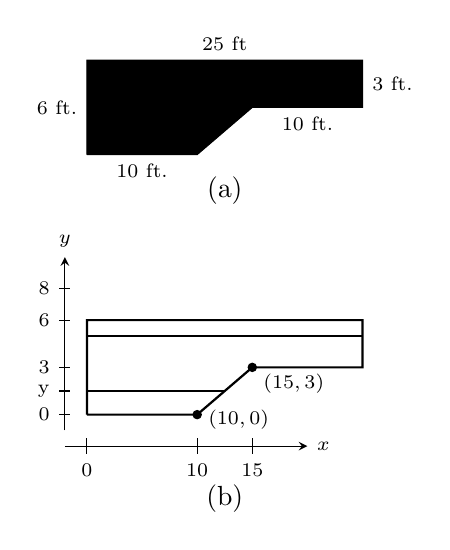
\begin{tikzpicture}[x=.14cm,y=.2cm,>=stealth]
  \draw [fill={\coloronefill}] (0,0)
   -- node [below] {\scriptsize 10 ft.} (10,0)
   -- node [below,yshift=-3ex] {(a)} (15,3)
   -- node [below] {\scriptsize 10 ft.} (25,3)
   -- node [right] {\scriptsize 3 ft.} (25,6)
   -- node [above] {\scriptsize 25 ft} (0,6)
   -- node [left] {\scriptsize 6 ft.} (0,0);
  \begin{scope}[yshift=-1.3in]
   \draw[>=stealth,->] (-2,-1) -- (-2,10) node [above] {\scriptsize $y$};
   \foreach \y/\x in {0/0,1.5/$y$,3/3,6/6,8/8}
   {
    \draw (-2.5,\y) node [left] {\scriptsize $\x$} -- (-1.5,\y);
   }
   \draw [thick] (0,0) --  (10,0) -- node [below,yshift=-7ex] {(b)} (15,3) --  (25,3)--  (25,6)-- (0,6) -- (0,0);
   \draw [thick,draw={\colorone}] (0,5) -- (25,5)
    (0,1.5) -- (12.5,1.5);
   \draw [fill=black] (10,0) circle (1.5pt) node [shift={(15pt,-2pt)}] {\scriptsize $(10,0)$}
    (15,3) circle (1.5pt) node [shift={(15pt,-6pt)}] {\scriptsize $(15,3)$};
   \draw[>=stealth,->] (-2,-2) -- (20,-2) node [right] {\scriptsize $x$};
   \foreach \y in {0,10,15}
   {
    \draw (\y,-2.5) node [below] {\scriptsize $\y$} -- (\y,-1.5);
   }
  \end{scope}
 \end{tikzpicture}
\end{tabular}}
\autoref{fig:pump3}(b) shows the pool oriented with this $y$-axis, along with 2 sample slices as the pool must be split into two different regions. 

The top region lies in the $y$-interval of $[3,6]$, where the length of the sample slice is $25$ ft as shown. As the pool is 20 ft wide, this sample slice of water has a volume of $V(y) = 20\cdot25\cdot dy$.  The water is to be pumped to a height of $y=8$, so the height function is $h(y) = 8-y$. The work done in pumping this top region of water is 
\[W_t = 62.4\int_3^6 500(8-y)\ dy = 327,600 \text{ ft-lb}.\]

The bottom region lies in the $y$-interval of $[0,3]$; we need to compute the length of the sample slice in this interval.

One end of the sample slice is at $x=0$ and the other is along the line segment joining the points $(10,0)$ and $(15,3)$. The equation of this line is $y= 3(x-10)/5$; as we will be integrating with respect to $y$, we rewrite this equation as $x=5y/3+10$. So the length of the sample slice is a difference of $x$-values: $x=0$ and $x=5y/3+10$, giving a length of $x=5y/3+10$. 

Again, as the pool is 20 ft wide, this slice of water has a volume of $V(y) = 20\cdot(5y/3+10)\cdot dy$; the height function is the same as before at $h(y)=8-y$. The work performed in emptying this part of the pool is
\[W_b = 62.4\int_0^3 20(5y/3+10)(8-y)\ dy = 299,520\ \text{ft-lb}.\]
The total work in emptying the pool is 
\[W = W_b+W_t = 327,600+299,520 = 627,120\ \text{ft-lb}.\]
Notice how the emptying of the bottom of the pool performs almost as much work as emptying the top. The top portion travels a shorter distance but has more water. In the end, this extra water produces more work.}

The next section introduces one final application of the definite integral, the calculation of fluid force on a plate.

\printexercises{exercises/07_05_exercises}
